\chapter{Bonsai Guidelines}
\label{chap:bonsai}
The implementation of the task described in Chapter \ref{chap:state_machine} was made with the Bonsai visual programming language. The goal of this chapter is to approach some aspects regarding the Bonsai implementation. However, a minimum degree of familiarity with the language will be assumed and the workflow will not be documented node by node.

When the workflow is first opened, the state machine schematized in Figure \ref{fig:state_machine} is easily identifiable. Here are some notes regarding the main workflow:
\begin{itemize}
    \item The states are implemented as SelectMany nodes;
    \item There is an additional SelectMany node that is responsible for outputting data from each trial;
    \item The last nodes of the state machine implementation are what allow the repetition of the workflow and, hence, to start a new trial;
    \item The initialization of variables, distributions and interface with hardware is implemented in GroupWorkflow nodes that aren't part of the state machine.
\end{itemize}

\section{State (SelectMany) Workflow Organization Logic}
\label{sec:state_organization}
It doesn't take much until a Bonsai workflow starts getting complex and, consequently, confusing. In order to improve the readability of the workflow (or at least try), a few guidelines are being followed so that any person that needs to look at the implementation of the task can easily understand it (and/or modify it):
\begin{itemize}
    \item In the main workflow, the inputs and outputs of each SelectMany node (i.e. each state) should be of the type Tuple<Boolean,int>. The idea is that the Boolean gives information regarding the validity of a trial, that is if a True comes out of a state the trial should proceed as planned, otherwise it should abort; and the int indicates the state from where the Tuple came from. Despite not being possible to abort a trial from every state, this guideline is a way to future-proof and standardize data-transfer between states.
    \item Separate independent functionality in a workflow (whether it is the main workflow or one of the SelectMany nodes) should be grouped in GroupWorkflow nodes and displayed in the first line of the workflow.
    \item If some logic is composed of multiple nodes and is used more than once, it should also be grouped in a GroupWorkflow node to avoid repetitions (example: TimestampEvent node).
    \item Since there is a sense of sequentiality of events throughtout the task, different branches of a workflow should be sorted from top to bottom by order of execution when possible.
\end{itemize}

\section{Timestamping Method}
\label{sec:timestamping}
In reaction time experiments, it is of extreme importance to timestamp every event with precision. A reliable way to timestamp each event is by using hardware timestamps (from the Harp Behavior board, to be exact).

Inside the SelectMany nodes where the different states are implemented, it is possible to find a node called TimestampEvent after events that need to be timestamped externally (i.e. non-Harp events). This node consists of a GroupWorkflow which, internally, receives an event from the outside and a hardware timestamp from the Timestamp subject (initialized in the Behavior GroupWorkflow), then ``zips'' both and sends the tuple to the CreateTimestamped node, which converts the tuple into a Bonsai.Harp.Timestamped<T> data type, and finally outputs it to the next node of the workflow. Figure \ref{fig:timestamp_event} shows the inside of the TimestampEvent node.

\begin{figure}[!ht]
    \centering
    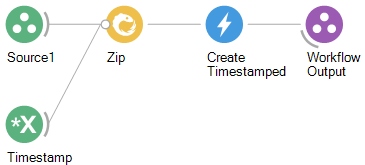
\includegraphics[width=0.3\textwidth]{Figures/timestamp_event.png}
    \caption{TimestampEvent GroupWorkflow ({\color{red} DEPRECATED})}
    \label{fig:timestamp_event}
\end{figure}